
在本章中，我们将证明\trFloerEquation{}的诸解空间具有一条\trRegularity{}性质。更确切地说，若 $H$ 是 $W$ 上的一个\trHamiltonian{}量，且 $x$ 与 $y$ 是 $H$ 的两条\trPeriodic\trTrajectory（\trPeriodic{}为 $1$），那么对每一个\trAlmostComplex{}结构 $J$，我们都可以考虑把\trTrajectory{} $x$ 连接到\trTrajectory{} $y$ 的\trFloerEquation{}诸解所成的空间 $\scr{M}(x,y)$。我们将证明：通过对 $H$ 取一个\trPerturbation（如有必要；且在 $x$ 与 $y$ 的附近不作修改，使得这两条\trTrajectory{}保持为\trPeriodic\trTrajectory），我们可以假设空间 $\scr{M}(x,y)$ 是一个维数为 $\mu(x)-\mu(y)$ 的\trManifold。其策略在于把空间 $\scr{M}(x,y)$ 描述成\trBanachManifold{} $\scr{P}(x,y)$（一个无穷维的\trBanachManifold）上某个\trVectorBundle{}的某个\trSection{}的零点所成之集。我们将利用\trSard{}定理的无穷维类比（即\trSard--\trSmale{}定理，亦即\cref{thm:sard-smale}）来证明：在对 $H$ 取\trPerturbation{}之后，空间 $\scr{M}(x,y)$ 是某个映射的一个\trRegularValue{}的\trPreimage。在这个框架下，应用\trSard{}定理需要假设诸\trTangentMap{}都是\trFredholmOperator。我们将证明这一性质并计算这些算子的\trIndex，它将是 $\mu(x)-\mu(y)$——也就是空间 $\scr{M}(x,y)$ 的维数。

\section{诸结果}
\label{sec:results}

我们使用\trFloer{}映射
\[
\begin{array}{c}
\scr{F}\colon\cC^{\infty}(\RR\times S^{1};W)\longrightarrow\cC^{\infty}(\RR\times S^{1};TW)\\[4pt]
u\longmapsto\dfrac{\partial u}{\partial s}+J\,\dfrac{\partial u}{\partial t}+\operatorname{grad}_{u}(H_{t})\text{，}
\end{array}
\]
或者更确切地说，是这个映射的一个 $W^{1,p}$ 版本（其细节我们将在\cref{subsec:banach-manifold-structure}中给出）。诸解所成的空间 $E=\cC^{\infty}(\RR\times S^{1};TW)$ 是一个\trVectorBundle{} $E\to\cC^{\infty}(\RR\times S^{1};W)$ 的全空间，它在 $u$ 处的\trFiber{} $E_{u}$ 由沿 $u$ 切于 $W$ 的诸\trVectorField{}组成。出于记号上的滥用，我们将写 $\scr{F}(u)=0$ 来表示 $\scr{F}(u)$ 落在 $E$ 的\trZeroSection{}之中。我们也可以使用\trEmbedding
\[
W\subset\RR^{m}\qquad\text{以及}\qquad TW\subset W\times\RR^{m}
\]
（从而避免这一记号滥用）。

注意到，倘若 $\scr{F}$ 与 $E$ 的\trZeroSection\trTransverse，那么\trFloerEquation{}的解空间就将是一个\trManifold。这种\trTransversality{}在\trZeroSection{}的\trPreimage{}中的一个解 $u$ 处，等价于从 $\mathrm{Im}(d\scr{F})_{u}$ 到\trFiber{} $E_{u}$ 上的投影之\trSurjective{}性。再一次出于记号上的滥用，我们将用记号 $(d\scr{F})_{u}$ 表示它与投影 $\mathrm{pr}_{E_{u}}$ 的复合。另一种选择是把 $\scr{F}$ 看成在 $\cC^{\infty}(\RR\times S^{1};\RR^{m})$ 中取值（参见\cref{sec:linearization-floer}）。

\trFloerEquation{}涉及一个\trAlmostComplex{}结构 $J$ 与一个\trHamiltonian{}量 $H$。我们的目标是选取 $H$ 的一个\trPerturbation（$J$ 固定），使得这条\trTransversality{}性质成立。我们将把满足这条性质的偶对 $(H,J)$ 称作\textbf{\trRegular}的（regular），并令 $(\scr{H}\times\scr{J})_{\mathrm{reg}}$ 表示全体\trRegular{}偶对所成之集。为了使 $(H,J)$ 成为\trRegular{}的，我们定义一个由 $H$ 的、与 $H$ 具有相同的\trPeriodic\trTrajectory{}的诸\trPerturbation{}所组成的\trBanachSpace{} $\cC^{\infty}_{\varepsilon}(H)$（\cref{sec:perturbations-h}）。然后我们将分两步给出证明：

\begin{itemize}
\item 我们将首先证明：对于\trHamiltonian{}量的一切\trPerturbation{}而言，从 $x$ 到 $y$ 的诸解所成的空间 $\scr{Z}(x,y,J)$ 是一个（无穷维的）\trBanachManifold。
\item 我们随后将证明\trSard--\trSmale{}定理可以应用于投影
\[
\pi\colon\scr{Z}(x,y,J)\longrightarrow\cC^{\infty}_{\varepsilon}(H)\text{，}
\]
这使我们得以结束证明，因为按定义
\[
\scr{M}(x,y,J,H)=\pi^{-1}(H)\text{。}
\]
\end{itemize}

在这两步中，\trLinearization{} $(d\scr{F})_{u}$ 的\trFredholm{}性质是决定性的。为了得到这条性质，我们必须把映射 $\scr{F}$ 的源空间与目标空间换成分别以 $W^{1,p}$ 与 $L^{p}$ \trSobolevSpace{}为模型的更大的\trBanachManifold。在这个框架下，我们将有
\[
(d\scr{F})_{u}\colon W^{1,p}(u^{\star}TW)\longrightarrow L^{p}(u^{\star}TW)
\]
（分别是沿 $u$ 切于 $W$ 的 $W^{1,p}$ 或 $L^{p}$ \trVectorField{}所成的空间，借助\trEmbedding{} $TW\subset W\times\RR^{m}$ 来定义；参见\cref{subsec:trajectory-spaces}）……其中，如前文所述，$(d\scr{F})_{u}$ 表示与到\trFiberBundle{} $E$ 的\trFiber{} $E_{u}$ 上的投影的复合，这一点我们将在\cref{sec:banach-manifold-p1p}中予以明确。诸结果如下。

\begin{theorem}\label{thm:regular-perturbations}
设 $H_{0}$ 是一个取定的\trNondegenerate{}\trHamiltonian{}量。则在 $\cC^{\infty}_{\varepsilon}(H_{0})$ 中存在 $0$ 的一个邻域，以及此邻域内诸\trDense\trOpen{}子集的一个可数交 $\scr{H}_{\mathrm{reg}}$，使得若 $h\in\scr{H}_{\mathrm{reg}}$，则 $H=H_{0}+h$ 是\trNondegenerate{}的，并且映射 $(d\scr{F})_{u}$ 对每个 $u\in\scr{M}(H_{0}+h,J)$ 都是\trSurjective{}的。
\end{theorem}

这里所用的\trNondegenerate{}性概念就是\cref{sec:hamiltonian-vector-fields}中所定义的那一个（\cref{thm:nondegenerate-periodic-solution}）。从这个结果出发，我们将推出本章的目标所在的下述结果。

\begin{theorem}\label{thm:moduli-manifold-dimension}
对每个 $h\in\scr{H}_{\mathrm{reg}}$ 以及 $H_{0}$ 的所有\trPeriodic{}为 $1$ 的\trContractible\trTrajectory{} $x$ 与 $y$，$\scr{M}(x,y,H_{0}+h)$ 是一个维数为 $\mu(x)-\mu(y)$ 的\trManifold。
\end{theorem}

\begin{proposition}\label{thm:z-banach-manifold}
令
\[
\scr{Z}(x,y,J)=\bigl\{(u,H=H_{0}+h)\ \bigm|\ h\in\cC^{\infty}_{\varepsilon}(H_{0})\ \text{且}\ u\in\scr{M}(x,y,J,H)\bigr\}\text{。}
\]
对 $x\ne y$，$\scr{Z}(x,y,J)$ 是一个（\trBanachManifold）。
\end{proposition}

这将是\trImplicitFunctionTheorem{}的一个推论，它来自下面这个以\trTransversality{}性质之名为人所知的结果。

\begin{proposition}\label{thm:transversality-property}
若 $(u,H)\in\scr{Z}(x,y)$，则
\[
\begin{array}{c}
\Gamma\colon W^{1,p}(\RR\times S^{1};\RR^{2n})\times\cC^{\infty}_{\varepsilon}(H_{0})\longrightarrow L^{p}(\RR\times S^{1};\RR^{2n})\\[4pt]
(Y,h)\longmapsto(d\scr{F}^{H})_{u}(Y)+\operatorname{grad}_{u}h
\end{array}
\]
（其中 $H=H_{0}+h$，而 $\scr{F}^{H}$ 是相应的\trFloer{}算子）是\trSurjective{}的，并且具有一个连续的右逆。
\end{proposition}

我们将在\cref{subsec:definition-gamma}中给出 $\Gamma$ 的定义的细节，特别是它确实定义在我们所考虑的那些空间之上这一事实。为了结束\cref{thm:regular-perturbations}与\cref{thm:moduli-manifold-dimension}的证明，我们还需要证明下面这个结果。

\begin{theorem}\label{thm:floer-map-fredholm}
对每个\trNondegenerate{}的\trHamiltonian{}量 $H$、每个受 $\omega$ \trCalibrated{}的\trAlmostComplex{}结构 $J$ 以及每个 $u\in\scr{M}(x,y,J,H)$，$(d\scr{F})_{u}$ 都是一个\trIndex{}为 $\mu(x)-\mu(y)$ 的\trFredholmOperator。
\end{theorem}

回顾一下：从一个\trBanachSpace{} $E$ 到一个\trBanachSpace{} $F$ 的（连续）\trLinearOperator{} $L\colon E\longrightarrow F$ 称作\trFredholmOperator，如果它的\trImage{}是闭的，并且它的\trKernel{}与\trCokernel{}都是有限维的。\trFredholmOperator{}的\trIndex{}是差
\[
\operatorname{Ind}L=\dim\operatorname{Ker}L-\dim\operatorname{Coker}L\text{。}
\]
从一个\trBanachSpace{}到另一个\trBanachSpace{}的可微映射称作\trFredholm{}映射，如果它在每一点处的\trDifferential{}都是一个\trFredholmOperator。\trFredholmOperator{}的各条有用的性质汇集于\cref{sec:appC-fredholm-theory}之中。

本章的结构如下：首先，我们利用\trSobolev{} $(1,p)$ 范数来描述我们所关心的那些\trTrajectory{}空间（在\cref{sec:banach-manifold-p1p}中）。然后我们定义\trHamiltonian{}量的\trPerturbation{}所成的\trBanachSpace（在\cref{sec:perturbations-h}中），此后我们便抵达证明本身：

\begin{itemize}
\item 在\cref{sec:linearization-floer}中，我们计算\trFloer{}映射的\trDifferential。
\item 在\cref{sec:transversality}中，我们证明\trTransversality{}性质（即\cref{thm:z-banach-manifold}与\cref{thm:transversality-property}），其间把\trFloerEquation{}诸解的几条性质当作已知的而暂置不论——这里要用到\trFloer{}映射的\trFredholm{}性质（此处即\cref{thm:floer-map-fredholm}）……
\item ……后者我们在\cref{sec:fredholm-property}中证明。
\item 在此之前，在\cref{sec:somewhere-injective}中，我们建立我们所用到的\trFloerEquation{}诸解的那些性质（“\trInjective{}性”、\trContinuationPrinciple）。
\item \trIndex{}的计算是\cref{sec:index-computation}的目标。
\item 在\cref{sec:exponential-decay}中，我们证明\trFloerEquation{}诸解在无穷远处（\trExponentialDecay）的一条本质性质。
\end{itemize}

我们本来也完全可以采用节序 8.4、8.7、8.8、8.9、8.6、8.5……
下面的示意图应当能帮助读者在本章诸陈述的迷宫中找到道路。

\begin{center}
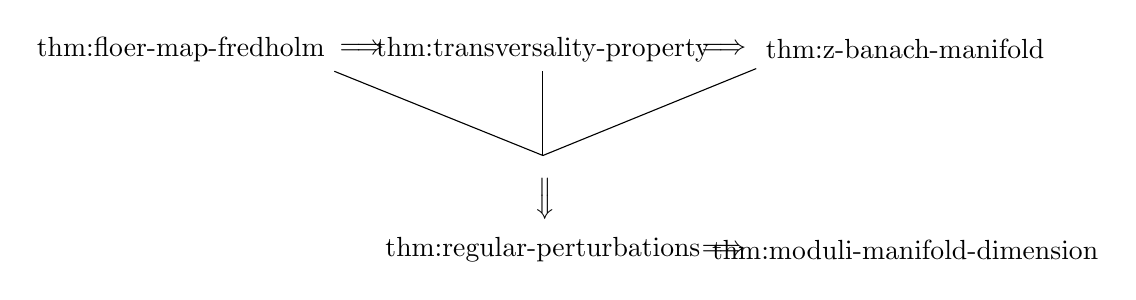
\begin{tikzpicture}
\node (thm815) at (-4.6,0) {\cref{thm:floer-map-fredholm}};
\node (prop814) at (0,0) {\cref{thm:transversality-property}};
\node (prop813) at (4.6,0) {\cref{thm:z-banach-manifold}};
\node (thm811) at (0,-2.55) {\cref{thm:regular-perturbations}};
\node (thm812) at (4.6,-2.55) {\cref{thm:moduli-manifold-dimension}};
\coordinate (mid) at (0,-1.35);
\draw (thm815.south east) -- (mid);
\draw (prop814.south) -- (mid);
\draw (prop813.south west) -- (mid);
\node at (-2.3,0) {$\Longrightarrow$};
\node at (2.3,0) {$\Longrightarrow$};
\node[rotate=-90] at (0,-1.9) {$\Longrightarrow$};
\node at (2.3,-2.55) {$\Longrightarrow$};
\end{tikzpicture}
\end{center}
